\documentclass[11pt,a4paper]{article}

\usepackage{Act}

\begin{document}
\input{\detokenize{/home/fenarius/Travail/Cours/cpge-info/latex/Macros.tex}}
\ModeExercice
\TD{18}{Modèle entité-association}
\newcommand{\SPATH}{/home/fenarius/Travail/Cours/cpge-info/docs/mp2i/files/C18/}


\psset{treesep=0.5cm,levelsep=0.8cm}

\setcounter{Exercise}{0}

\begin{Exercise}[title={Cinémas}, origin={\bac \; {\sc ccinp} sujet zéro}]\\
    On considère la base de données décrite par le modèle entité-association suivant :
    \begin{center}
        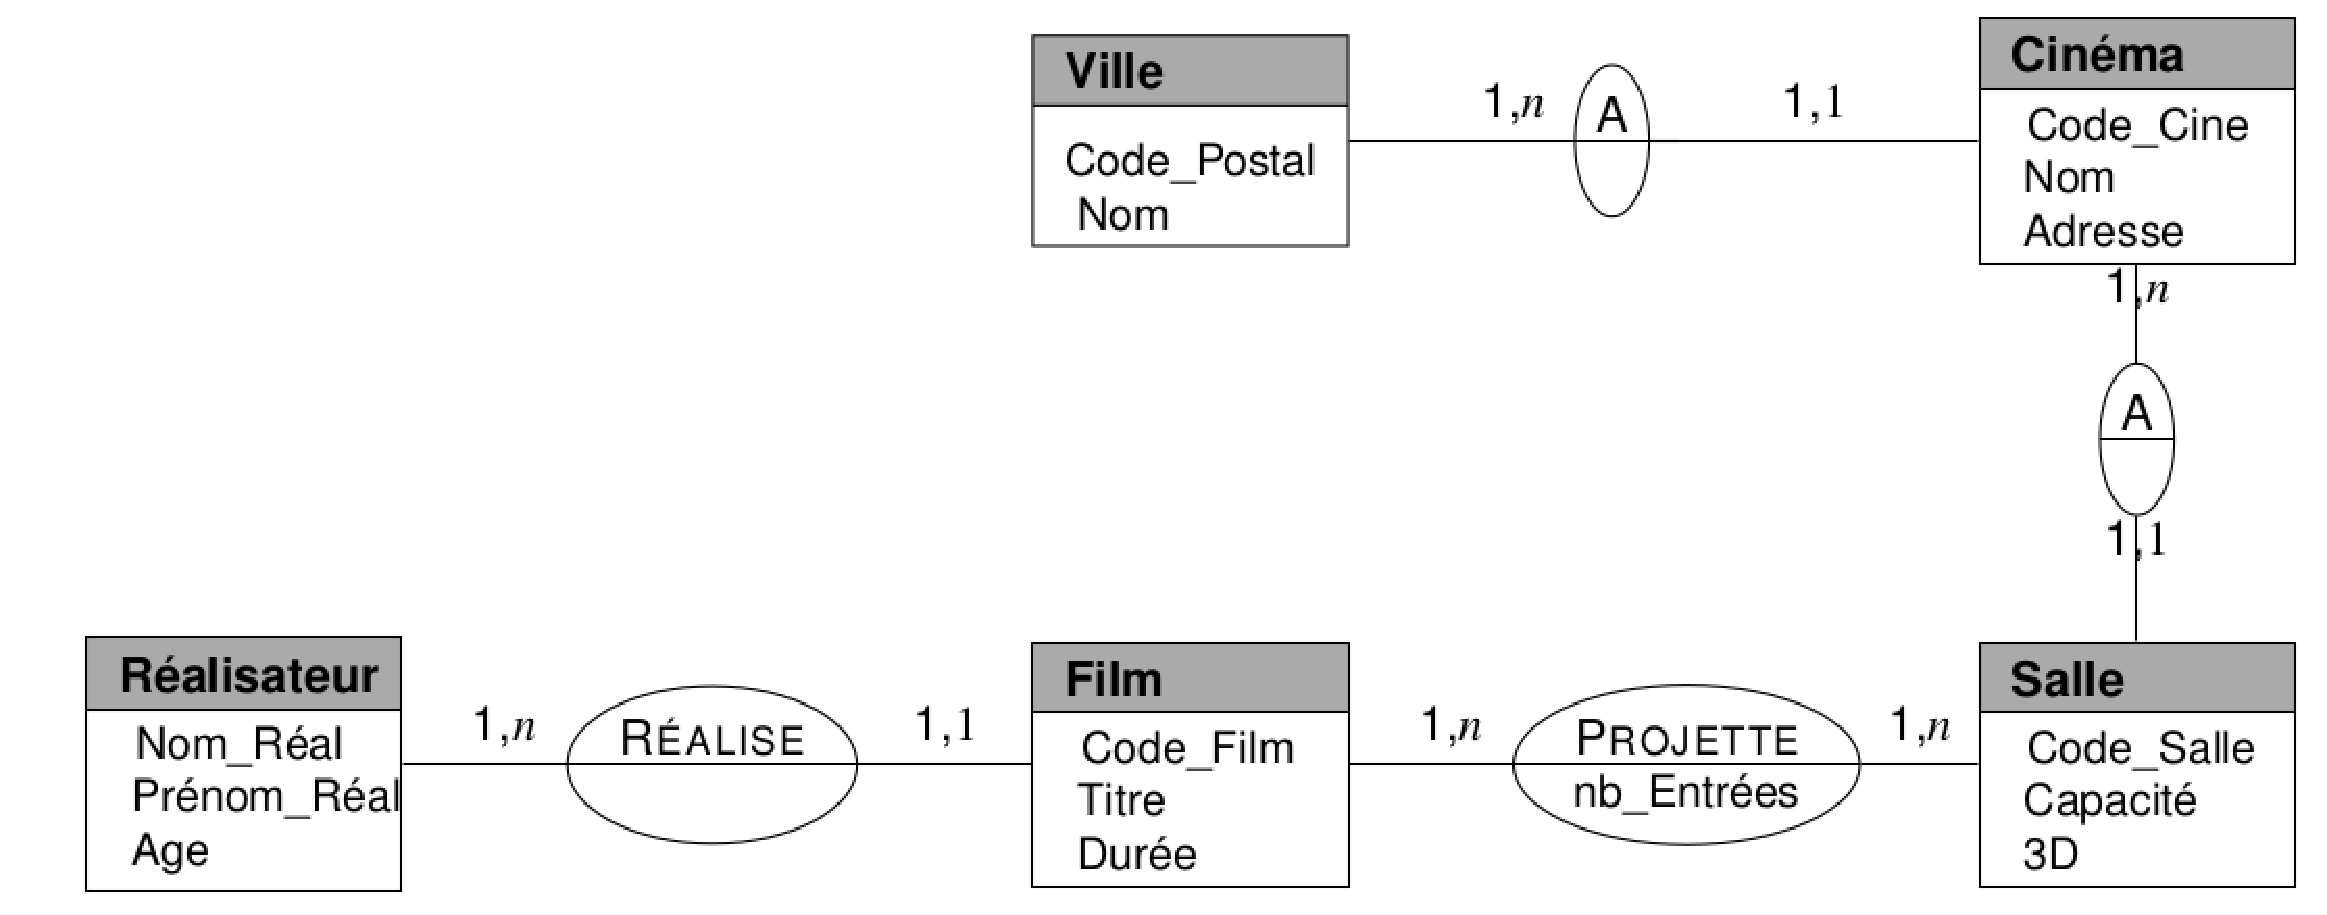
\includegraphics[width=400px]{ea1.eps}
    \end{center}
    Dans cette représentation, on lie des entités par des associations avec des cardinalités. Ainsi par exemple 
    \begin{center}
        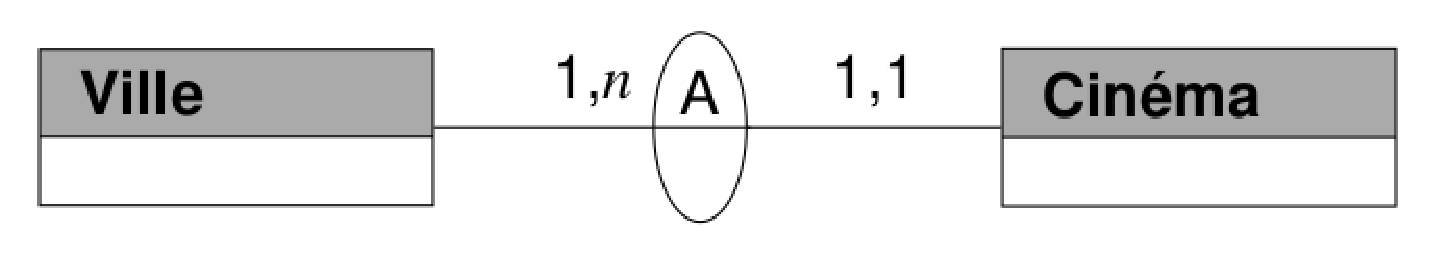
\includegraphics[height=40px]{ea2.eps}
    \end{center}
    peut se lire comme \og{} \textit{Une ville a 1 à n cinéma(s)} \fg{} et \og{} \textit{un cinéma est présent dans une et une seule ville} \fg{}. Parfois, l'association possède des propriétés (le nombre d'entrées d'un film projeté dans une salle par exemple).
    \smallskip
    On suppose que le champ {\sc 3d} de l'entité Salle est un entier, valant 0 si la salle n'est pas en {\sc 3d} et 1 sinon. On suppose de plus que la durée des films est en heures. Enfin, on affirme qu'une ville peut-être uniquement déterminé par son code postal et son nom.
    \Question{Donner le schéma relationnel correspondant. Préciser les clés primaires et étrangères des relations. Les clés primaires peuvent être associées à plusieurs attributs.}
    \Question{Ecrire les requêtes suivantes en langage {\sc sql} :}
    \subQuestion{Donner le titre des films durant moins de 2h.}
    \subQuestion{Donner le nom et le prénom du réalisateur ayant réalisé le film \og{} Matrix \fg{}.}
    \subQuestion{Compter le nombre de cinémas à Nantes.}
    \subQuestion{Donner l'adresse des cinémas contenant au moins une salle {\sc 3d}.}
    \subQuestion{Donner le code des films projetés dans toutes les salles.}
    \subQuestion{Donner la liste des titres des films projetés dans le cinéma \og{} Le Rio \fg{}.}

\end{Exercise}


\end{document}